% =============================================================================
% CHAPTER 17: DIE INTERVENTIONSLOGIK
% =============================================================================
%------------------------------------------------------------------------------
% Chapter 17: Die Interventionslogik (Master Chapter)
%------------------------------------------------------------------------------
% Version: 2.0 (January 2026)
%
% Purpose: Master Chapter explaining the complete intervention logic that
%          emerges from the 10C Framework. Serves as foundation for all
%          subsequent intervention chapters (18-20).
%
% Primary Appendix: HHH - METHOD-TOOLKIT (20-Field Schema, Theorems HHH-T1-T8)
% Secondary Appendices: III (R-Score), BA (Segments), BB (Equilibria), G (Glossary)
%
% Prerequisites: Chapters 1-16 (complete 10C Framework understanding)
% Leads to: Ch18 (Journey), Ch19 (Segments), Ch20 (Portfolios)
%
% Chapter Type: C (Application)
%------------------------------------------------------------------------------
% =============================================================================

\chapter{Die Interventionslogik}
\label{ch:intervention-logic}

% -----------------------------------------------------------------------------
% QUICK REFERENCE BOX
% -----------------------------------------------------------------------------
\begin{tcolorbox}[colback=blue!5!white, colframe=blue!75!black,
    title=Zentrale Begriffe in diesem Kapitel]
\small
\begin{tabular}{@{}ll@{}}
\textbf{Archetyp} & 6-dimensionale Interventions-Klassifikation \\
\textbf{6D-Raum} & Type $\times$ Scope $\times$ Level $\times$ FEPSDE $\times$ Phase $\times$ Awareness \\
\textbf{$\gamma(\Psi)$-Filter} & Kontextabhängige Feasibility-Prüfung \\
\textbf{20-Field Schema} & Standardisierte Interventions-Spezifikation \\
\textbf{R-Score} & Relevanz-Score für GO/PILOT/NO-GO Entscheidungen \\
\textbf{EMP/THR/EXP} & Epistemic Status von Archetypen \\
\end{tabular}
\end{tcolorbox}

% -----------------------------------------------------------------------------
% APPENDIX REFERENCES BOX
% -----------------------------------------------------------------------------
\begin{tcolorbox}[colback=gray!5!white, colframe=gray!75!black,
    title=Appendix-Referenzen]

\textbf{Primär:} Appendix HHH (METHOD-TOOLKIT) --- Theoreme HHH-T1 bis T8, 20-Field Schema, Feasibility-Reduktion

\textbf{10C COREs (Emergenz):}
\begin{itemize}[nosep]
\item AAA (WHO), C (WHAT), B (HOW), V (WHEN), BBB (WHERE)
\item AU (AWARE), AV (READY), AW (STAGE), HI (HIERARCHY)
\end{itemize}

\textbf{Unterstützend:}
\begin{itemize}[nosep]
\item III (METHOD-LLMMC-CAL): R-Score und GO/PILOT/NO-GO Entscheidungen
\item BA (FORMAL-SEGMENT): Segment-Targeting (F9)
\item BB (FORMAL-EQUILIBRIA): Interventions-Gleichgewichte
\item G (REF-GLOSSARY): Begriffsdefinitionen
\end{itemize}

\textbf{Daten:}
\begin{itemize}[nosep]
\item \texttt{data/gamma\_matrix\_complete.json}: $\gamma(\Psi \rightarrow \text{FEPSDE})$ Matrix
\item \texttt{docs/frameworks/core-framework-definition.yaml}: 10C SSOT
\end{itemize}

\end{tcolorbox}

% -----------------------------------------------------------------------------
% INTUITION BOX
% -----------------------------------------------------------------------------
\begin{tcolorbox}[colback=yellow!5!white, colframe=yellow!75!black,
    title=Intuition: Anna und das Interventions-Dilemma]

Anna leitet das Präventionsprogramm einer Schweizer Krankenkasse. Ihr Ziel: Die Diabetes-Prävalenz unter 45-65-Jährigen um 20\% senken.

Sie steht vor einem klassischen Problem:
\begin{itemize}[nosep]
\item \textbf{14,400 theoretische Möglichkeiten}: Welche Intervention? Welcher Typ? Für wen? Wann?
\item \textbf{Begrenzte Ressourcen}: CHF 500,000 Budget, 18 Monate Zeit
\item \textbf{Keine Garantie}: Manche Interventionen könnten nach hinten losgehen
\end{itemize}

Dieses Kapitel gibt Anna---und allen Interventions-Designern---ein \textbf{systematisches Framework}, das aus dem 10C-Modell emergiert und evidenzbasierte Entscheidungen ermöglicht.

\textit{Am Ende dieses Kapitels wird Anna wissen, wie sie von 14,400 Möglichkeiten zu einer priorisierten Shortlist mit GO/PILOT/NO-GO Empfehlungen kommt.}
\end{tcolorbox}

% -----------------------------------------------------------------------------
% CENTRAL QUESTION BOX
% -----------------------------------------------------------------------------
\begin{tcolorbox}[colback=red!5!white, colframe=red!75!black,
    title=Die Zentrale Frage]
\textbf{Wie können wir systematisch Interventionen designen, die kontextabhängig, evidenzbasiert und kombinierbar sind?}

Und spezifischer:
\begin{enumerate}[nosep]
\item Woher kommen die Interventionskategorien? (Emergenz aus 10C)
\item Wie reduzieren wir 14,400 theoretische Archetypen auf praktikable Optionen?
\item Wie dokumentieren wir Interventionen standardisiert?
\item Wie treffen wir GO/PILOT/NO-GO Entscheidungen?
\end{enumerate}
\end{tcolorbox}

% -----------------------------------------------------------------------------
% CHAPTER OVERVIEW
% -----------------------------------------------------------------------------
\begin{tcolorbox}[colback=green!5!white, colframe=green!75!black,
    title=Kapitelübersicht]

Dieses Kapitel ist das \textbf{Master-Kapitel} für verhaltensökonomische Interventionen. Es erklärt die gesamte Interventionslogik; die Folgekapitel vertiefen einzelne Aspekte.

\begin{enumerate}
\item \textbf{Teil 0} (Section~\ref{sec:17-status-quo}): \textbf{10C Status Quo Assessment} (NEU)
    \begin{itemize}[nosep]
    \item Diagnose VOR Intervention (aus Kapitel 1--16)
    \item Der 10C Status Quo Vektor $\vec{S}_0$
    \item Intervention als 10C-Transformation: $\vec{S}_0 \mapsto \vec{S}_1$
    \end{itemize}
\item \textbf{Teil I} (Section~\ref{sec:17-foundation}): Theoretische Fundierung
    \begin{itemize}[nosep]
    \item Emergenz aus 10C Framework
    \item Der 14,400 Archetypen-Raum
    \item Die $\gamma(\Psi)$-Reduktion
    \end{itemize}
\item \textbf{Teil II} (Section~\ref{sec:17-types}): Die 8 Interventionstypen
\item \textbf{Teil III} (Section~\ref{sec:17-schema}): Das 20-Field Schema
\item \textbf{Teil IV} (Section~\ref{sec:17-dimensions}): Die 5 Anwendungsdimensionen
    \begin{itemize}[nosep]
    \item Vorschau auf Kapitel 18 (Phase), 19 (Segment), 20 (Portfolio)
    \end{itemize}
\item \textbf{Teil V} (Section~\ref{sec:17-process}): Der Entscheidungsprozess
\item \textbf{Teil VI} (Section~\ref{sec:17-examples}): Worked Examples
\item \textbf{Teil VII} (Section~\ref{sec:17-summary}): Zusammenfassung und Reading Path
\end{enumerate}
\end{tcolorbox}


%%%%%%%%%%%%%%%%%%%%%%%%%%%%%%%%%%%%%%%%%%%%%%%%%%%%%%%%%%%%%%%%%%%%%%%%%%%%%%%
%%%%%%%%%%%%%%%%%%%%%%%%%%%%%%%%%%%%%%%%%%%%%%%%%%%%%%%%%%%%%%%%%%%%%%%%%%%%%%%
%%  TEIL 0: 10C STATUS QUO ASSESSMENT (VOR INTERVENTION)
%%%%%%%%%%%%%%%%%%%%%%%%%%%%%%%%%%%%%%%%%%%%%%%%%%%%%%%%%%%%%%%%%%%%%%%%%%%%%%%
%%%%%%%%%%%%%%%%%%%%%%%%%%%%%%%%%%%%%%%%%%%%%%%%%%%%%%%%%%%%%%%%%%%%%%%%%%%%%%%

\section{10C Status Quo Assessment: Der Ausgangspunkt}
\label{sec:17-status-quo}

\begin{tcolorbox}[colback=blue!5!white, colframe=blue!75!black,
    title=\textbf{KRITISCH: Diagnose VOR Intervention}]
\textbf{Keine Intervention ohne 10C Status Quo Assessment!}

Die Kapitel 1--16 etablieren das vollständige 10C CORE Framework. \textbf{Bevor} wir intervenieren, müssen wir den aktuellen Zustand in allen 9 Dimensionen diagnostizieren.
\end{tcolorbox}

\subsection{Die 10C Status Quo Checkliste}

Für jede Zielgruppe/Situation muss der aktuelle Zustand erfasst werden:

\begin{table}[htbp]
\centering
\caption{10C Status Quo Assessment: Diagnose vor Intervention}
\label{tab:17-9c-status-quo}
\renewcommand{\arraystretch}{1.4}
\footnotesize
\begin{tabular}{@{}llll@{}}
\toprule
\textbf{CORE} & \textbf{Diagnose-Frage} & \textbf{Quelle (Kap.)} & \textbf{Output} \\
\midrule
\textbf{WHO} (AAA) & Auf welchem Level agiert die Zielgruppe? & Ch.\ 5, App.\ AAA & $L \in \{1,2,3,4\}$ \\
\textbf{WHAT} (C) & Welche FEPSDE-Dimensionen sind relevant? & Ch.\ 10, App.\ C & $d \in \{F,E,P,S,D,X\}$ \\
\textbf{HOW} (B) & Welche $\gamma$-Strukturen existieren aktuell? & Ch.\ 5, App.\ B & $\gamma_{\text{current}}$ \\
\textbf{WHEN} (V) & Welcher Kontext $\Psi$ liegt vor? & Ch.\ 9, App.\ V & $\Psi = (\Psi_E, ..., \Psi_X)$ \\
\textbf{WHERE} (BBB) & Welche Parameter sind bekannt? & Ch.\ 4, App.\ BBB & $\Theta_{\text{known}}$ \\
\textbf{AWARE} (AU) & Wie hoch ist die aktuelle Awareness? & Ch.\ 11, App.\ AU & $A_0 \in [0,1]$ \\
\textbf{READY} (AV) & Wie hoch ist die aktuelle Willingness? & Ch.\ 12, App.\ AV & $W_0 \in [0,1]$ \\
\textbf{STAGE} (AW) & In welcher Journey-Phase befindet sich die Zielgruppe? & Ch.\ 13, App.\ AW & $\varphi_0 \in \{1,...,5\}$ \\
\textbf{HIERARCHY} (HI) & Auf welcher Entscheidungsebene? & Ch.\ 1b, App.\ HI & Scope $\in \{L0,...,L3\}$ \\
\bottomrule
\end{tabular}
\end{table}

\subsection{Der 10C Status Quo Vektor}

Das Assessment produziert einen \textbf{10C Status Quo Vektor}:
\begin{equation}
\boxed{\vec{S}_0 = (L, d, \gamma_{\text{current}}, \Psi, \Theta, A_0, W_0, \varphi_0, \text{Scope})}
\label{eq:17-status-quo-vector}
\end{equation}

Dieser Vektor ist der \textbf{Input} für alle Interventions-Entscheidungen.

\subsection{Intervention als 10C-Transformation}

Eine Intervention $\mathcal{I}$ ist formal eine \textbf{Transformation} des Status Quo Vektors:
\begin{equation}
\boxed{\mathcal{I}: \vec{S}_0 \mapsto \vec{S}_1 = \vec{S}_0 + \Delta\vec{S}(\mathcal{I})}
\label{eq:17-intervention-transform}
\end{equation}

Wobei $\Delta\vec{S}(\mathcal{I})$ der \textbf{10C Delta Vektor} ist---die erwartete Veränderung in jeder Dimension.

\subsection{Welche Intervention verändert welche 10C-Dimension?}

\begin{table}[htbp]
\centering
\caption{Interventionstypen und ihre primären 10C-Zieldimensionen}
\label{tab:17-type-to-9c}
\renewcommand{\arraystretch}{1.3}
\small
\begin{tabular}{@{}llll@{}}
\toprule
\textbf{Typ} & \textbf{Primäre 10C-Dimension} & \textbf{Sekundäre} & \textbf{$\Delta$-Richtung} \\
\midrule
T1: Awareness & \textbf{AWARE} (AU) & READY & $A \uparrow$ \\
T2: Feedback & \textbf{AWARE} (AU), \textbf{READY} (AV) & STAGE & $A \uparrow, W \uparrow$ \\
T3: Kontextuell & \textbf{WHEN} (V) & HOW & $\Psi \rightarrow \Psi'$ \\
T4: Temporal & \textbf{WHEN} (V), \textbf{STAGE} (AW) & --- & $\Psi_T \uparrow, \varphi \uparrow$ \\
T5: Identität & \textbf{WHO} (AAA), \textbf{WHAT} (C) & READY & $L \rightarrow L', W_{\text{base}} \uparrow$ \\
T6: Sozial & \textbf{WHAT} (C) & WHO & $u_S \uparrow$ \\
T7: Finanziell & \textbf{WHAT} (C) & --- & $u_F \uparrow$ \\
T8: Bindung & \textbf{HOW} (B) & STAGE & $\gamma_{ij} \rightarrow \gamma'_{ij}$ \\
\bottomrule
\end{tabular}
\end{table}

\begin{tcolorbox}[colback=green!5!white, colframe=green!75!black,
    title=Der vollständige Interventions-Zyklus]
\begin{center}
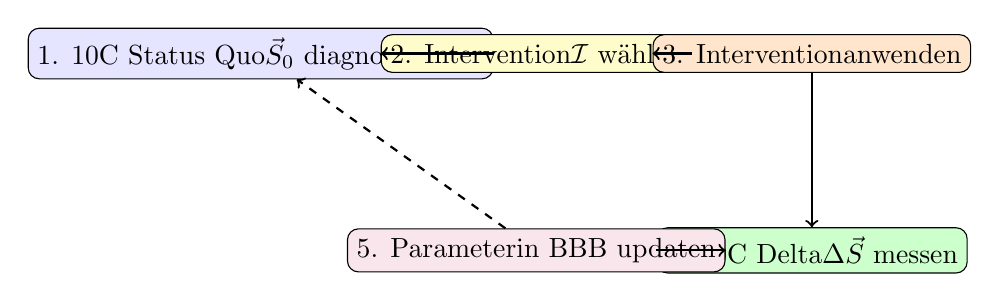
\begin{tikzpicture}[node distance=2.5cm, auto]
\node[draw, rounded corners, fill=blue!10, minimum width=3.5cm] (diag) {1. 10C Status Quo\\$\vec{S}_0$ diagnostizieren};
\node[draw, rounded corners, fill=yellow!20, minimum width=3.5cm, right of=diag, xshift=1cm] (select) {2. Intervention\\$\mathcal{I}$ wählen};
\node[draw, rounded corners, fill=orange!20, minimum width=3.5cm, right of=select, xshift=1cm] (apply) {3. Intervention\\anwenden};
\node[draw, rounded corners, fill=green!20, minimum width=3.5cm, below of=apply] (measure) {4. 10C Delta\\$\Delta\vec{S}$ messen};
\node[draw, rounded corners, fill=purple!10, minimum width=3.5cm, left of=measure, xshift=-1cm] (learn) {5. Parameter\\in BBB updaten};

\draw[->, thick] (diag) -- (select);
\draw[->, thick] (select) -- (apply);
\draw[->, thick] (apply) -- (measure);
\draw[->, thick] (measure) -- (learn);
\draw[->, thick, dashed] (learn) -- (diag);
\end{tikzpicture}
\end{center}

\textbf{Der Learning Loop:} Gemessene $\Delta\vec{S}$ fließen zurück in Appendix BBB (WHERE) und verbessern zukünftige Vorhersagen.
\end{tcolorbox}


%%%%%%%%%%%%%%%%%%%%%%%%%%%%%%%%%%%%%%%%%%%%%%%%%%%%%%%%%%%%%%%%%%%%%%%%%%%%%%%
%%%%%%%%%%%%%%%%%%%%%%%%%%%%%%%%%%%%%%%%%%%%%%%%%%%%%%%%%%%%%%%%%%%%%%%%%%%%%%%
%%  TEIL I: THEORETISCHE FUNDIERUNG
%%%%%%%%%%%%%%%%%%%%%%%%%%%%%%%%%%%%%%%%%%%%%%%%%%%%%%%%%%%%%%%%%%%%%%%%%%%%%%%
%%%%%%%%%%%%%%%%%%%%%%%%%%%%%%%%%%%%%%%%%%%%%%%%%%%%%%%%%%%%%%%%%%%%%%%%%%%%%%%

\section{Theoretische Fundierung}
\label{sec:17-foundation}

Interventionen im EBF-Framework sind keine ad-hoc Maßnahmen. Sie \textbf{emergieren systematisch} aus dem 10C CORE Framework. Diese theoretische Fundierung unterscheidet EBF von pragmatischen ``Nudge-Katalogen''.

\subsection{Von 10C zu 6D: Die Emergenz der Klassifikationsdimensionen}
\label{sec:17-emergence}

Jede der 10C CORE-Fragen generiert eine Klassifikationsdimension für Interventionen. Sechs dieser Dimensionen bilden den \textbf{6D-Klassifikationsraum} (Theorem HHH-T7).

\begin{tcolorbox}[colback=blue!5!white, colframe=blue!75!black,
    title=\textbf{Die 6D-Emergenz aus 10C}]

\begin{center}
\renewcommand{\arraystretch}{1.3}
\begin{tabular}{@{}llcll@{}}
\toprule
\textbf{CORE} & \textbf{Frage} & \textbf{Theorem} & \textbf{Dimension} & \textbf{Kategorien} \\
\midrule
--- & $W_{\text{eff}}$ Decomposition & HHH-T1 & \textbf{Type} & 8 \\
HIERARCHY (HI) & Welche Entscheidungsebene? & HHH-T2 & \textbf{Scope} & 5 \\
WHO (AAA) & Wer hat Utility? & HHH-T3 & \textbf{Level} & 4 \\
WHAT (C) & Was ist Utility? & HHH-T4 & \textbf{Dimension} & 6 \\
STAGE (AW) & Wo in der Journey? & HHH-T5 & \textbf{Phase} & 5 \\
AWARE (AU) & Wie bewusst? & HHH-T6 & \textbf{Awareness} & 3 \\
\bottomrule
\end{tabular}
\end{center}

\textbf{Theorem HHH-T7 (Complete Classification):} Jede Intervention ist vollständig klassifiziert durch:
\begin{equation}
\boxed{\mathcal{I} \mapsto (\text{Type}, \text{Scope}, \text{Level}, \text{Dimension}, \text{Phase}, \text{Awareness})}
\label{eq:17-6d-classification}
\end{equation}

\end{tcolorbox}

% -----------------------------------------------------------------------------
% 10C INTEGRATION MATRIX (Added for 10C Compliance)
% -----------------------------------------------------------------------------
\begin{tcolorbox}[colback=purple!5!white, colframe=purple!75!black,
    title=\textbf{10C CORE Integration Matrix}]

Die Interventionslogik emergiert aus allen 10C CORE Fragen. Diese Matrix zeigt die systematische Verbindung:

\begin{center}
\renewcommand{\arraystretch}{1.3}
\footnotesize
\begin{tabular}{@{}llll@{}}
\toprule
\textbf{CORE} & \textbf{Frage} & \textbf{Interventions-Dimension} & \textbf{Appendix} \\
\midrule
\textbf{WHO} (AAA) & Wer hat Utility? & Level: IND, Dyadic, Group, Societal & AAA \\
\textbf{WHAT} (C) & Was ist Utility? & FEPSDE: F, E, P, S, D, X & C \\
\textbf{HOW} (B) & Wie interagieren? & $\gamma_{ij}$: Komplementarität zwischen $\mathcal{I}$ & B \\
\textbf{WHEN} (V) & Wann zählt Kontext? & 8Ψ: $\Psi_E, \Psi_S, \Psi_T, \Psi_P, \Psi_I, \Psi_C, \Psi_D, \Psi_X$ & V \\
\textbf{WHERE} (BBB) & Woher die Zahlen? & Parameter: $\alpha, \sigma, \gamma$ aus Literatur & BBB \\
\textbf{AWARE} (AU) & Wie bewusst? & Awareness-Regime: Low/Medium/Full & AU \\
\textbf{READY} (AV) & Handlungsbereit? & $W_{\text{eff}}$: Effective Willingness & AV \\
\textbf{STAGE} (AW) & Wo in der Journey? & Phase: 1-5 der BCJ & AW \\
\textbf{HIERARCHY} (HI) & Wie stratifiziert? & Scope: Instant→System (L3→L0) & HI \\
\bottomrule
\end{tabular}
\end{center}

\textbf{Emergenz-Kette:}
\begin{equation}
\text{10C CORE} \xrightarrow{\text{HHH-T1 bis T8}} \text{6D Klassifikation} \xrightarrow{\gamma(\Psi)\text{-Filter}} \text{Feasible Archetypen}
\end{equation}

\end{tcolorbox}

\subsubsection{Dimension 1: Type (aus $W_{\text{eff}}$)}

Die 8 Interventionstypen emergieren aus der Zerlegung der Effective Willingness Funktion (Theorem HHH-T1):
\begin{equation}
W_{\text{eff}} = W_{\text{base}} \cdot A(\cdot) \cdot (1 + \kappa_{AWX}) \cdot (1 + \kappa_{KON}) \cdot (1 + \kappa_{JNY})
\label{eq:17-weff}
\end{equation}

Jede Komponente, die modifiziert werden kann, definiert einen Interventionstyp:
\begin{center}
\small
\begin{tabular}{@{}clll@{}}
\toprule
\# & \textbf{Typ} & \textbf{Target} & \textbf{Formel} \\
\midrule
1 & Awareness & $A(\cdot)$ & $A \mapsto A'$ \\
2 & Feedback & $\kappa_{AWX}$ & $\kappa_{AWX} \mapsto \kappa'_{AWX}$ \\
3 & Kontextuell & $\kappa_{KON}$ & $\kappa_{KON} \mapsto \kappa'_{KON}$ \\
4 & Temporal & $\kappa_{JNY}$ & $\kappa_{JNY} \mapsto \kappa'_{JNY}$ \\
5 & Identität & $W_{\text{base}}$ & $W_{\text{base}} \mapsto W'_{\text{base}}$ \\
6 & Sozial & $u_S$ & $u_S \mapsto u'_S$ \\
7 & Finanziell & $u_F$ & $u_F \mapsto u'_F$ \\
8 & Bindung & $\gamma_{ij}$ & $\gamma_{ij} \mapsto \gamma'_{ij}$ \\
\bottomrule
\end{tabular}
\end{center}

\subsubsection{Dimension 2: Scope (aus HIERARCHY)}

Die 5 temporalen Scopes emergieren aus der Entscheidungshierarchie (Theorem HHH-T2):
\begin{center}
\begin{tabular}{@{}lll@{}}
\toprule
\textbf{Scope} & \textbf{Hierarchy Level} & \textbf{Zeithorizont} \\
\midrule
Instant & L3 (Emergent) & Stunden--Tage \\
Operative & L3 (Emergent) & Tage--Wochen \\
Tactical & L2 (Derived) & Wochen--Monate \\
Strategic & L1 (Strategic Roots) & Monate--Jahre \\
System & L0 (Operative) & Jahre--Dekaden \\
\bottomrule
\end{tabular}
\end{center}

\subsubsection{Dimension 3: Level (aus WHO)}

Die 4 Target-Levels emergieren aus der Welfare Hierarchy (Theorem HHH-T3):
\begin{center}
\begin{tabular}{@{}ll@{}}
\toprule
\textbf{Level} & \textbf{Definition} \\
\midrule
Individual (L1) & Einzelperson als Target \\
Dyadic (L2) & Zweierbeziehung (z.B. Arzt-Patient) \\
Group (L3) & Gruppe/Team/Familie \\
Societal (L4) & Gesellschaft/Population \\
\bottomrule
\end{tabular}
\end{center}

\subsubsection{Dimension 4: FEPSDE (aus WHAT)}

Die 6 Utility-Dimensionen emergieren aus dem FEPSDE-Framework (Theorem HHH-T4):
\begin{center}
\begin{tabular}{@{}ll@{}}
\toprule
\textbf{Dimension} & \textbf{Beispiel-Interventionen} \\
\midrule
Financial (F) & Incentives, Steuern, Subventionen \\
Emotional (E) & Framing, Affekt-Priming \\
Physical (P) & Gesundheitsprogramme, Ergonomie \\
Social (S) & Normen, Peer-Effekte \\
Development (D) & Bildung, Skill-Building \\
Existential (X) & Sinn-Interventionen, Werte \\
\bottomrule
\end{tabular}
\end{center}

\subsubsection{Dimension 5: Phase (aus STAGE)}

Die 5 Journey-Phasen emergieren aus der Behavioral Change Journey (Theorem HHH-T5):
\begin{center}
\begin{tabular}{@{}lll@{}}
\toprule
\textbf{Phase} & \textbf{$S(t)$ Range} & \textbf{Charakteristik} \\
\midrule
Awareness & $[0, 0.2)$ & Problem noch nicht erkannt \\
Trigger & $[0.2, 0.4)$ & Problem erkannt, noch keine Handlung \\
Action & $[0.4, 0.6)$ & Erste Verhaltensänderung \\
Maintenance & $[0.6, 0.8)$ & Verhalten wird gehalten \\
Stabilization & $[0.8, 1.0]$ & Verhalten ist Habit/Identität \\
\bottomrule
\end{tabular}
\end{center}

\subsubsection{Dimension 6: Awareness (aus AWARE)}

Die 3 Awareness-Regimes emergieren aus der Awareness-Funktion (Theorem HHH-T6):
\begin{center}
\begin{tabular}{@{}lll@{}}
\toprule
\textbf{Regime} & \textbf{$A(\cdot)$ Range} & \textbf{Implikation} \\
\midrule
Low & $A < 0.3$ & Awareness-Intervention nötig \\
Medium & $0.3 \leq A < 0.7$ & Standard-Interventionen möglich \\
Full & $A \geq 0.7$ & Awareness-Intervention redundant \\
\bottomrule
\end{tabular}
\end{center}


\subsection{Der 14,400 Archetypen-Raum}
\label{sec:17-14400}

Die Kombination der 6 Dimensionen erzeugt einen theoretischen Raum von:
\begin{equation}
\boxed{8 \times 5 \times 4 \times 6 \times 5 \times 3 = 14{,}400 \text{ Interventions-Archetypen}}
\label{eq:17-14400}
\end{equation}

\begin{tcolorbox}[colback=yellow!5!white, colframe=yellow!75!black,
    title=Warum so viele?]
Jeder Archetyp ist eine spezifische Kombination:
\begin{quote}
``Eine \textit{Feedback}-Intervention (Type) mit \textit{taktischem} Horizont (Scope), die auf \textit{Individuen} (Level) in der \textit{Physical}-Dimension (FEPSDE) während der \textit{Action}-Phase (Phase) bei \textit{mittlerer} Awareness (Awareness) zielt.''
\end{quote}

Dies ist Archetyp $(2, 3, 1, 3, 3, 2)$ im 6D-Raum.
\end{tcolorbox}

\textbf{Das Problem:} 14,400 Optionen sind unpraktikabel. Wir brauchen eine prinzipiengeleitete Reduktion.


\subsection{Die Elegante Reduktion: Der $\gamma(\Psi)$-Filter}
\label{sec:17-reduction}

\begin{tcolorbox}[colback=green!5!white, colframe=green!75!black,
    title=\textbf{Theorem HHH-T8: Feasibility Constraint System}]

Ein Archetyp $\vec{a} = (t, s, l, d, \varphi, A)$ ist \textbf{feasible} genau dann, wenn:
\begin{equation}
\boxed{\text{Feasible}(\vec{a}) \iff C_{\text{affinity}} \wedge C_{\text{logical}} \wedge C_{\text{scale}} \wedge C_{\text{empirical}}}
\label{eq:17-feasibility}
\end{equation}

\end{tcolorbox}

\subsubsection{Die Vier Constraint-Klassen}

\begin{enumerate}
\item \textbf{$C_{\text{affinity}}$: Affinitäts-Constraints}

Manche Type-Phase Kombinationen haben geringe Wirksamkeit:
\begin{equation}
C_{\text{affinity}}(\vec{a}) \iff \alpha_{t,\varphi} \geq \theta_\alpha \quad \text{(Default: } \theta_\alpha = 0.4\text{)}
\end{equation}

\textit{Beispiel:} Awareness-Interventionen in der Stabilization-Phase haben $\alpha \approx 0.2$ (redundant).

\item \textbf{$C_{\text{logical}}$: Logische Constraints}

Manche Kombinationen sind logisch widersprüchlich:
\begin{align}
&\neg(\varphi = \text{Awareness} \wedge A = \text{Full}) \tag{Redundanz} \\
&\neg(s = \text{System} \wedge l = \text{Individual}) \tag{Skalen-Mismatch}
\end{align}

\item \textbf{$C_{\text{scale}}$: Skalen-Kohärenz}

Scope und Level müssen kompatibel sein:
\begin{equation}
C_{\text{scale}}(\vec{a}) \iff |s_{\text{rank}} - l_{\text{rank}}| \leq 2
\end{equation}

\item \textbf{$C_{\text{empirical}}$: Evidenz-Constraints}

Manche (Type, Dimension) Paarungen haben keine Evidenzbasis.

\textbf{ACHTUNG:} Dies ist der risikoreichste Constraint---siehe Section~\ref{sec:17-epistemic}.
\end{enumerate}

\subsubsection{Der $\gamma(\Psi)$-Filter}

Die eleganteste Reduktion nutzt die \textbf{kontextabhängige Komplementaritätsmatrix}:
\begin{equation}
\boxed{\text{Feasible}(\mathcal{I} | \Psi) \iff \gamma(\Psi \rightarrow \text{target\_FEPSDE}(\mathcal{I})) \geq \theta}
\label{eq:17-gamma-filter}
\end{equation}

Die $\gamma$-Matrix ist geschätzt via LLM Monte Carlo (Appendix CAL1) und gespeichert in:
\begin{center}
\texttt{data/gamma\_matrix\_complete.json}
\end{center}

\subsubsection{Reduktions-Pipeline}

\begin{table}[htbp]
\centering
\caption{Die Reduktions-Pipeline: Von 14,400 zu $\approx$2,000}
\label{tab:17-reduction-pipeline}
\renewcommand{\arraystretch}{1.3}
\begin{tabular}{@{}clcc@{}}
\toprule
\textbf{Stage} & \textbf{Constraint} & \textbf{Output} & \textbf{Status} \\
\midrule
0 & 10C Framework & 6 Dimensionen & Emergent \\
1 & Kombinatorik & 14,400 & Emergent \\
2 & $C_{\text{affinity}}$ & $\approx$8,000 & Annahme (A2, A3) \\
3 & $C_{\text{logical}}$ & $\approx$5,000 & Emergent \\
4 & $C_{\text{scale}}$ & $\approx$3,500 & Annahme (A4) \\
5 & $C_{\text{empirical}}$ & $\approx$2,500 & Annahme (A5) \\
6 & $\gamma(\Psi)$-Filter & $\approx$2,000 & Annahme (A6, A7) \\
\bottomrule
\end{tabular}
\end{table}


\subsection{Epistemische Ehrlichkeit: Emergent vs. Annahmen}
\label{sec:17-epistemic}

Wissenschaftliche Integrität erfordert Transparenz darüber, was \textit{abgeleitet} ist und was \textit{angenommen} wird.

\subsubsection{Die Annahmen-Register (A1--A7)}

\begin{table}[htbp]
\centering
\caption{Explizite Annahmen in der Reduktions-Pipeline}
\label{tab:17-assumptions}
\renewcommand{\arraystretch}{1.3}
\small
\begin{tabular}{@{}clll@{}}
\toprule
\textbf{ID} & \textbf{Annahme} & \textbf{Risiko} & \textbf{Mitigation} \\
\midrule
A1 & Kardinalitäten (5 Phases, 3 Awareness) & Niedrig & Granularität erhöhen \\
A2 & Affinitäts-Matrix Werte & Mittel & Empirisch kalibrieren \\
A3 & Threshold $\theta_\alpha = 0.4$ & Mittel & $\theta_\alpha$ anpassen \\
A4 & Scale-Kohärenz $\leq 2$ & Niedrig & Lockern für Innovation \\
A5 & Empirische Evidenz erforderlich & \textbf{Hoch} & 3-Tier Klassifikation \\
A6 & $\gamma$-Matrix Werte (LLMMC) & Mittel & Konfidenzintervalle \\
A7 & Threshold $\theta = 0.3$ & Mittel & Konservativ wählen \\
\bottomrule
\end{tabular}
\end{table}

\subsubsection{Archetype Epistemic Classification}

\begin{tcolorbox}[colback=orange!5!white, colframe=orange!75!black,
    title=\textbf{Die Drei-Tier Archetype-Klassifikation}]

Analog zu den Parameter-Level Epistemic Tags (Appendix EST) klassifizieren wir Archetypen:

\begin{center}
\renewcommand{\arraystretch}{1.3}
\begin{tabular}{@{}lp{6cm}l@{}}
\toprule
\textbf{Status} & \textbf{Kriterium} & \textbf{Aktion} \\
\midrule
\cellcolor{green!20}\textbf{EMP-Archetype} & Kombination empirisch getestet mit positivem Effekt & $\rightarrow$ Scale \\
\cellcolor{blue!20}\textbf{THR-Archetype} & Theoretisch plausibel, aber Kombination nicht getestet & $\rightarrow$ Pilot \\
\cellcolor{orange!20}\textbf{EXP-Archetype} & Neue Kombination, keine Evidenz & $\rightarrow$ Experiment \\
\bottomrule
\end{tabular}
\end{center}

\textbf{Kritische Unterscheidung:} Ein Archetyp kann \texttt{[EMP]}-Parameter verwenden, aber trotzdem \texttt{THR-Archetype} sein, wenn die \textit{Kombination} nie getestet wurde.

\end{tcolorbox}

\begin{tcolorbox}[colback=red!5!white, colframe=red!75!black,
    title=\textbf{Warnung: Absence of Evidence $\neq$ Evidence of Absence}]

Der Empirical Constraint (A5) hat das höchste Risiko für \textbf{False Negatives}:
\begin{itemize}[nosep]
\item Neue Kombinationen werden ausgeschlossen
\item Innovation wird systematisch unterdrückt
\end{itemize}

\textbf{Empfehlung:} Verwende $C_{\text{empirical}}$ NICHT als harten Filter, sondern nur für die EMP/THR/EXP Klassifikation.

\end{tcolorbox}


%%%%%%%%%%%%%%%%%%%%%%%%%%%%%%%%%%%%%%%%%%%%%%%%%%%%%%%%%%%%%%%%%%%%%%%%%%%%%%%
%%%%%%%%%%%%%%%%%%%%%%%%%%%%%%%%%%%%%%%%%%%%%%%%%%%%%%%%%%%%%%%%%%%%%%%%%%%%%%%
%%  TEIL II: DIE 8 INTERVENTIONSTYPEN
%%%%%%%%%%%%%%%%%%%%%%%%%%%%%%%%%%%%%%%%%%%%%%%%%%%%%%%%%%%%%%%%%%%%%%%%%%%%%%%
%%%%%%%%%%%%%%%%%%%%%%%%%%%%%%%%%%%%%%%%%%%%%%%%%%%%%%%%%%%%%%%%%%%%%%%%%%%%%%%

\section{Die 8 Interventionstypen}
\label{sec:17-types}

Jeder Interventionstyp zielt auf eine spezifische Komponente der $W_{\text{eff}}$-Funktion (Gleichung~\ref{eq:17-weff}).

\subsection{Typ 1: Awareness-Interventionen ($\rightarrow A$)}
\label{sec:17-type-awareness}

\textbf{Mechanismus:} Wissensvermittlung---Informationslücken schließen, die informierte Entscheidungen verhindern.

\textbf{Beispiele:}
\begin{itemize}[nosep]
\item Nährwertangaben auf Lebensmitteln
\item Warnhinweise auf Zigarettenpackungen
\item Energieeffizienz-Labels
\item Finanzielle Bildungsprogramme
\end{itemize}

\textbf{Wann wirksam:} Wenn die Zielgruppe relevante Informationen nicht hat und ihr Verhalten bei Wissen ändern würde.

\textbf{Wann nicht wirksam:} Wenn Awareness nicht das Problem ist. Raucher wissen, dass Rauchen schädlich ist---mehr Information hilft nicht.

\textbf{EBF-Verbindung:} $A(\cdot) \mapsto A'(\cdot)$ in der $W_{\text{eff}}$-Gleichung.


\subsection{Typ 2: Feedback-Interventionen ($\rightarrow \kappa_{AWX}$)}
\label{sec:17-type-feedback}

\textbf{Mechanismus:} Echtzeit-Information über Verhalten und Konsequenzen, die Selbstkorrektur ermöglicht.

\textbf{Beispiele:}
\begin{itemize}[nosep]
\item Smart-Meter Energieanzeigen
\item Fitness-Tracker und Schrittzähler
\item Ausgaben-Alerts von Banken
\item Geschwindigkeitsanzeigen auf Straßen
\end{itemize}

\textbf{Wann wirksam:} Wenn Menschen keine genaue Intuition über ihr Verhalten haben und es bei Wissen anpassen würden.

\textbf{Wann nicht wirksam:} Wenn Feedback zu verzögert oder komplex ist, um darauf zu reagieren.

\textbf{EBF-Verbindung:} $\kappa_{AWX} \mapsto \kappa'_{AWX}$---Awareness-Willingness-Action Kopplung.


\subsection{Typ 3: Kontextuelle Interventionen ($\rightarrow \kappa_{KON}$)}
\label{sec:17-type-contextual}

\textbf{Mechanismus:} Choice Architecture---die Umgebung so verändern, dass gewünschtes Verhalten einfacher und ungewünschtes schwerer wird.

\textbf{Beispiele:}
\begin{itemize}[nosep]
\item Default-Einschreibung in Altersvorsorge \citep{madrian2001}
\item Opt-out Organspende-Systeme
\item Kleinere Teller in Kantinen
\item Automatische Erhöhung der Sparrate
\end{itemize}

\textbf{Wann wirksam:} Wenn Friktion eine Hauptbarriere ist und die Zielgruppe ``passiv'' ist---bereit, Defaults zu akzeptieren.

\textbf{Wann nicht wirksam:} Wenn starke Präferenzen Defaults überschreiben, oder wenn die strukturelle Änderung Reaktanz auslöst.

\textbf{EBF-Verbindung:} $\kappa_{KON} \mapsto \kappa'_{KON}$---Kontext-Kopplung, insbesondere $\Psi_I$ (institutionelle Defaults).


\subsection{Typ 4: Temporale Interventionen ($\rightarrow \kappa_{JNY}$)}
\label{sec:17-type-temporal}

\textbf{Mechanismus:} Strategischer Einsatz von Zeit---Deadlines, Cooling-off Perioden, Timing von Prompts.

\textbf{Beispiele:}
\begin{itemize}[nosep]
\item Bedenkzeit bei großen Käufen
\item Steuer-Deadlines
\item ``Letzte Chance''-Dringlichkeit
\item Optimales Timing von Erinnerungen (Zahltag für Spar-Prompts)
\end{itemize}

\textbf{Wann wirksam:} Wenn Timing die Entscheidungsqualität beeinflusst oder Dringlichkeit/Geduld strategisch induziert werden kann.

\textbf{Wann nicht wirksam:} Wenn künstliche Dringlichkeit als Manipulation wahrgenommen wird.

\textbf{EBF-Verbindung:} $\kappa_{JNY} \mapsto \kappa'_{JNY}$---Journey-Kopplung, interagiert mit $\Psi_T$ (temporaler Kontext).


\subsection{Typ 5: Identitäts-Interventionen ($\rightarrow W_{\text{base}}$)}
\label{sec:17-type-identity}

\textbf{Mechanismus:} Aktivierung oder Umformung des Selbstkonzepts, um Verhalten mit Identität in Einklang zu bringen.

\textbf{Beispiele:}
\begin{itemize}[nosep]
\item ``Sei ein Wähler'' vs. ``Wähle'' Framing \citep{bryan2011}
\item ``Du bist der Typ Mensch, der...'' Botschaften
\item Vorbilder-Programme
\item Identitäts-Labels (``Du bist Umweltschützer'')
\end{itemize}

\textbf{Wann wirksam:} Wenn Identität formbar ist und das Zielverhalten als konsistent mit einer wünschenswerten Identität geframed werden kann.

\textbf{Wann nicht wirksam:} Wenn Identität fixiert ist oder die vorgeschlagene Identität mit dem bestehenden Selbstkonzept kollidiert.

\textbf{EBF-Verbindung:} $W_{\text{base}} \mapsto W'_{\text{base}}$---die persistenteste Form der Verhaltensänderung via $IDN^L$.


\subsection{Typ 6: Soziale Interventionen ($\rightarrow u_S$)}
\label{sec:17-type-social}

\textbf{Mechanismus:} Aktivierung sozialer Normen---was andere tun (deskriptiv) oder was andere gutheißen (injunktiv).

\textbf{Beispiele:}
\begin{itemize}[nosep]
\item ``9 von 10 Nachbarn recyceln'' (deskriptive Norm)
\item Hotel-Handtuch-Wiederverwendung mit Gäste-Referenz
\item Steuercompliance-Botschaften (``Die meisten zahlen pünktlich'')
\item Wahl-Erinnerungen mit Gemeinschafts-Referenz
\end{itemize}

\textbf{Wann wirksam:} Wenn die Zielgruppe sozial orientiert ist und die Norm das gewünschte Verhalten unterstützt.

\textbf{Wann nicht wirksam:} Wenn die Zielgruppe autonomieorientiert ist (Reaktanz) oder die tatsächliche Norm der Botschaft widerspricht.

\textbf{EBF-Verbindung:} $u_S \mapsto u'_S$---aktiviert $U^{IDN}$ aus dem FEPSDE-Framework.


\subsection{Typ 7: Finanzielle Interventionen ($\rightarrow u_F$)}
\label{sec:17-type-financial}

\textbf{Mechanismus:} Finanzielle Belohnungen oder Strafen, die die Kosten-Nutzen-Rechnung verändern.

\textbf{Beispiele:}
\begin{itemize}[nosep]
\item CO2-Steuern
\item Spar-Matching-Programme
\item Pay-for-Performance im Gesundheitswesen
\item Subventionen für Elektrofahrzeuge
\end{itemize}

\textbf{Wann wirksam:} Wenn finanzielle Überlegungen zentral für die Entscheidung sind und der Anreiz groß genug ist.

\textbf{Wann nicht wirksam:} Wenn intrinsische Motivation stark ist---Bezahlung kann interne Motivation ``verdrängen'' (Crowding-out).

\textbf{EBF-Verbindung:} $u_F \mapsto u'_F$. Der Crowding-out Effekt reflektiert $\gamma < 0$ mit sozialen Interventionen.

\begin{tcolorbox}[colback=red!5!white, colframe=red!75!black,
    title=Warnung: Crowding Out]
\textbf{Vorsicht bei der Kombination von Incentives mit sozialen/Identitäts-Interventionen.}

Wenn Menschen etwas tun, weil es ``das Richtige'' ist (intrinsische Motivation), kann Bezahlung signalisieren, dass es eigentlich eine Transaktion ist, keine moralische Handlung. Die intrinsische Motivation verschwindet, und wenn die Bezahlung stoppt, stoppt auch das Verhalten.

\textbf{Faustregel:} Bezahle Menschen nicht für Dinge, die sie ohnehin aus sozialen oder Identitätsgründen tun würden.
\end{tcolorbox}


\subsection{Typ 8: Bindungs-Interventionen ($\rightarrow \gamma_{ij}$)}
\label{sec:17-type-binding}

\textbf{Mechanismus:} Pre-Commitment Devices, die zukünftiges Verhalten festlegen und Present Bias überwinden.

\textbf{Beispiele:}
\begin{itemize}[nosep]
\item Fitnessstudio-Verträge mit Kündigungsstrafen
\item Spar-Commitment-Konten \citep{ashraf2006}
\item Öffentliche Zielankündigungen
\item Implementation Intentions (``Ich werde am Montag um 7 Uhr trainieren'')
\end{itemize}

\textbf{Wann wirksam:} Wenn Present Bias ($\beta < 1$) das Problem ist und die Person ein ``Sophisticate'' ist, der seine Selbstkontrollprobleme erkennt.

\textbf{Wann nicht wirksam:} Wenn die Person ein ``Naif'' ist, der seinen Present Bias nicht erkennt (wird kein Commitment suchen).

\textbf{EBF-Verbindung:} $\gamma_{ij} \mapsto \gamma'_{ij}$---verändert die Komplementaritätsstruktur zwischen Perioden.


\subsection{Hybride Interventionen}
\label{sec:17-type-hybrid}

\textbf{Definition:} Eine hybride Intervention $\mathcal{I}_H$ modifiziert mehrere Komponenten gleichzeitig:
\begin{equation}
\mathcal{I}_H = \mathcal{I}_1 \circ \mathcal{I}_2 \circ \ldots \circ \mathcal{I}_k \quad \text{wobei } k \geq 2
\end{equation}

Die Effektivität hängt von der Komplementarität ab:
\begin{equation}
E(\mathcal{I}_H) = \sum_{i} E(\mathcal{I}_i) + \sum_{i < j} \gamma_{ij} \cdot \sqrt{E(\mathcal{I}_i) \cdot E(\mathcal{I}_j)}
\end{equation}

\textbf{Wichtig:} Hybride sind KEINE primitiven Typen, sondern Kompositionen. Die Beweislast liegt bei der Hybrid-Intervention:
\begin{itemize}[nosep]
\item \textbf{Null-Hypothese:} Einzelne Mechanismen reichen aus
\item \textbf{Alternative:} Multi-Mechanismus erforderlich
\item \textbf{Test:} Nur kombinieren, wenn einzelne Mechanismen nachweislich versagen
\end{itemize}


\subsection{Zusammenfassung: Die 8 Typen im Überblick}

\begin{table}[htbp]
\centering
\caption{Die 8 Interventionstypen}
\label{tab:17-types-summary}
\renewcommand{\arraystretch}{1.3}
\small
\begin{tabular}{@{}clllc@{}}
\toprule
\textbf{\#} & \textbf{Typ} & \textbf{Target} & \textbf{Mechanismus} & \textbf{Typische Phase} \\
\midrule
1 & Awareness & $A(\cdot)$ & Information & Awareness \\
2 & Feedback & $\kappa_{AWX}$ & Selbstkorrektur & Action \\
3 & Kontextuell & $\kappa_{KON}$ & Choice Architecture & Action \\
4 & Temporal & $\kappa_{JNY}$ & Timing & Variabel \\
5 & Identität & $W_{\text{base}}$ & Selbstkonzept & Stabilization \\
6 & Sozial & $u_S$ & Normen & Awareness, Action \\
7 & Finanziell & $u_F$ & Incentives & Action \\
8 & Bindung & $\gamma_{ij}$ & Pre-Commitment & Trigger \\
\bottomrule
\end{tabular}
\end{table}


%%%%%%%%%%%%%%%%%%%%%%%%%%%%%%%%%%%%%%%%%%%%%%%%%%%%%%%%%%%%%%%%%%%%%%%%%%%%%%%
%%%%%%%%%%%%%%%%%%%%%%%%%%%%%%%%%%%%%%%%%%%%%%%%%%%%%%%%%%%%%%%%%%%%%%%%%%%%%%%
%%  TEIL III: DAS 20-FIELD SCHEMA
%%%%%%%%%%%%%%%%%%%%%%%%%%%%%%%%%%%%%%%%%%%%%%%%%%%%%%%%%%%%%%%%%%%%%%%%%%%%%%%
%%%%%%%%%%%%%%%%%%%%%%%%%%%%%%%%%%%%%%%%%%%%%%%%%%%%%%%%%%%%%%%%%%%%%%%%%%%%%%%

\section{Das 20-Field Schema}
\label{sec:17-schema}

Das 20-Field Schema ist die \textbf{standardisierte Spezifikationssprache} für Interventionen. Es stellt sicher, dass alle relevanten Aspekte dokumentiert werden.

\subsection{Struktur: Drei Tiers}

Die 20 Felder sind in drei epistemische Tiers organisiert:

\begin{table}[htbp]
\centering
\caption{Die Drei-Tier Struktur des 20-Field Schemas}
\label{tab:17-tiers}
\renewcommand{\arraystretch}{1.3}
\small
\begin{tabular}{@{}clll@{}}
\toprule
\textbf{Tier} & \textbf{Status} & \textbf{Felder} & \textbf{Herkunft} \\
\midrule
1 & Emergent & F2, F4, F5, F6, F12, (+F21) & 10C via Theoreme \\
2 & Operational & F7, F8, F11, F14, F15 & Design-Parameter \\
3 & Interface & F9, F10 & Links zu anderen Appendices \\
--- & Administrativ & F1, F13, F16-F20 & Dokumentation \\
\bottomrule
\end{tabular}
\end{table}


\subsection{Tier 1: Emergente Felder}

Diese Felder emergieren direkt aus dem 10C Framework:

\begin{center}
\renewcommand{\arraystretch}{1.3}
\begin{tabular}{@{}llll@{}}
\toprule
\textbf{Field} & \textbf{Name} & \textbf{CORE} & \textbf{Optionen} \\
\midrule
F2 & Intervention Type & $W_{\text{eff}}$ & 8 Typen \\
F4 & Target Structure & WHO (AAA) & IND, IDN, Collective \\
F5 & FEPSDE Dimension & WHAT (C) & F, E, P, S, D, X \\
F6 & Journey Phase & STAGE (AW) & 5 Phasen \\
F12 & Temporal Scope & HIERARCHY (HI) & 5 Scopes \\
\bottomrule
\end{tabular}
\end{center}


\subsection{Tier 2: Operationale Felder}

Diese Felder sind Design-Parameter (Forschungsfragen RQ-1 bis RQ-4 in Appendix HHH prüfen Emergenz-Potenzial):

\begin{center}
\renewcommand{\arraystretch}{1.3}
\begin{tabular}{@{}lll@{}}
\toprule
\textbf{Field} & \textbf{Name} & \textbf{Optionen} \\
\midrule
F7 & Framing Logic & Positive, Negative, Social, Neutral \\
F8 & Autonomy Level & Voluntary, Default, Mandate, Prohibition \\
F11 & Side Effect Risk & Low, Medium, High \\
F14 & Path Function & Door-opener, Amplifier, Escalator, Stabilizer \\
F15 & Repetition & One-time, Cyclic, Continuous \\
\bottomrule
\end{tabular}
\end{center}


\subsection{Tier 3: Interface-Felder}

Diese Felder verlinken zu anderen Framework-Komponenten:

\begin{center}
\renewcommand{\arraystretch}{1.3}
\begin{tabular}{@{}llll@{}}
\toprule
\textbf{Field} & \textbf{Name} & \textbf{Verlinkt zu} & \textbf{Funktion} \\
\midrule
F9 & Target Segment & Appendix PAP1 & Segment-ID \\
F10 & Complementarity & Appendix HOW & $\gamma$-Werte zu anderen Interventionen \\
\bottomrule
\end{tabular}
\end{center}


\subsection{Administrative Felder}

\begin{center}
\renewcommand{\arraystretch}{1.3}
\small
\begin{tabular}{@{}lll@{}}
\toprule
\textbf{Field} & \textbf{Name} & \textbf{Zweck} \\
\midrule
F1 & Title/Label & Menschenlesbare Bezeichnung \\
F13 & Evaluation Plan & Messungs-Strategie \\
F16 & Responsible Role & Verantwortlichkeit \\
F17 & Source/Evidence & Literatur-Referenzen \\
F18 & System Link/ID & Technische Integration \\
F19 & Description & Mechanismus-Erklärung \\
F20 & Status & Planned/Tested/Active/Rejected \\
\bottomrule
\end{tabular}
\end{center}


\subsection{Application Depths}
\label{sec:17-depths}

Das Schema unterstützt drei Anwendungstiefen:

\begin{tcolorbox}[colback=green!5!white, colframe=green!75!black,
    title=Light Mode: F1--F6 (10 Minuten)]
\textbf{Wann:} Rapid Screening, initiale Ideation

\textbf{Felder:}
\begin{itemize}[nosep]
\item F1: Titel
\item F2: Typ (einer der 8)
\item F3: Kontext-Level (State/Org/Individual/Digital)
\item F4: Target (IND/IDN/Collective)
\item F5: FEPSDE-Dimension
\item F6: Journey-Phase
\end{itemize}

\textbf{Test:} Wenn du F1--F6 nicht in 10 Minuten ausfüllen kannst, verstehst du deine Intervention nicht gut genug.
\end{tcolorbox}

\begin{tcolorbox}[colback=yellow!5!white, colframe=yellow!75!black,
    title=Hybrid Mode: F1--F12 (30 Minuten)]
\textbf{Wann:} Standard-Interventionsdesign, Steering-Committee Präsentation

\textbf{Zusätzliche Felder:}
\begin{itemize}[nosep]
\item F7: Framing Logic
\item F8: Autonomy Level
\item F9: Target Segment
\item F10: Complementarity
\item F11: Side Effect Risk
\item F12: Temporal Scope
\end{itemize}
\end{tcolorbox}

\begin{tcolorbox}[colback=blue!5!white, colframe=blue!75!black,
    title=Profound Mode: F1--F20 (60 Minuten)]
\textbf{Wann:} Research-Grade Dokumentation, High-Stakes Interventionen

\textbf{Zusätzliche Felder:}
\begin{itemize}[nosep]
\item F13--F20: Evaluation, Path Function, Repetition, Responsibility, Evidence, System Link, Description, Status
\end{itemize}
\end{tcolorbox}


%%%%%%%%%%%%%%%%%%%%%%%%%%%%%%%%%%%%%%%%%%%%%%%%%%%%%%%%%%%%%%%%%%%%%%%%%%%%%%%
%%%%%%%%%%%%%%%%%%%%%%%%%%%%%%%%%%%%%%%%%%%%%%%%%%%%%%%%%%%%%%%%%%%%%%%%%%%%%%%
%%  TEIL IV: DIE 5 ANWENDUNGSDIMENSIONEN
%%%%%%%%%%%%%%%%%%%%%%%%%%%%%%%%%%%%%%%%%%%%%%%%%%%%%%%%%%%%%%%%%%%%%%%%%%%%%%%
%%%%%%%%%%%%%%%%%%%%%%%%%%%%%%%%%%%%%%%%%%%%%%%%%%%%%%%%%%%%%%%%%%%%%%%%%%%%%%%

\section{Die 5 Anwendungsdimensionen}
\label{sec:17-dimensions}

Interventions-Design erfordert Entscheidungen in 5 Dimensionen. Dieses Kapitel gibt einen Überblick; die Folgekapitel vertiefen.

\begin{table}[htbp]
\centering
\caption{Die 5 Anwendungsdimensionen}
\label{tab:17-dimensions}
\renewcommand{\arraystretch}{1.3}
\begin{tabular}{@{}llll@{}}
\toprule
\textbf{Dimension} & \textbf{Frage} & \textbf{Vertiefung} & \textbf{Key Construct} \\
\midrule
TYPE & WAS wirkt? & Dieses Kapitel (§\ref{sec:17-types}) & 8 Typen aus $W_{\text{eff}}$ \\
PHASE & WANN einsetzen? & Kapitel 18 & Phase-Type Affinity \\
SEGMENT & FÜR WEN? & Kapitel 19 & Segment Multiplier $\sigma_s$ \\
PORTFOLIO & WIE kombinieren? & Kapitel 20 & $\gamma$-Matrix \\
CONTEXT & UNTER WELCHEN Bedingungen? & Verteilt ($\Psi$) & 8 $\Psi$-Dimensionen \\
\bottomrule
\end{tabular}
\end{table}


\subsection{Phase-Dimension (Vorschau Kapitel 18)}

Die Phase-Type Affinity Matrix zeigt, welche Interventionstypen in welcher Journey-Phase am effektivsten sind:

\begin{center}
\small
\renewcommand{\arraystretch}{1.2}
\begin{tabular}{@{}lccccc@{}}
\toprule
\textbf{Type} & \textbf{Awareness} & \textbf{Trigger} & \textbf{Action} & \textbf{Maintenance} & \textbf{Stabilization} \\
\midrule
Awareness & \cellcolor{green!30}0.9 & 0.6 & 0.3 & 0.2 & 0.1 \\
Feedback & 0.3 & 0.5 & \cellcolor{green!30}0.9 & \cellcolor{green!30}0.8 & 0.5 \\
Kontextuell & 0.2 & \cellcolor{green!30}0.8 & \cellcolor{green!30}0.9 & 0.7 & 0.5 \\
Identität & 0.2 & 0.3 & 0.4 & 0.6 & \cellcolor{green!30}0.9 \\
\bottomrule
\end{tabular}
\end{center}

\textbf{Kapitel 18} vertieft: Path Functions, Sequenzierung, Phase-Diagnose.


\subsection{Segment-Dimension (Vorschau Kapitel 19)}

Dieselbe Intervention kann bei verschiedenen Segmenten sehr unterschiedlich wirken:

\begin{equation}
E_{\text{segment}}(\mathcal{I}) = E_{\text{base}}(\mathcal{I}) \times \sigma_s
\end{equation}

wobei $\sigma_s \in [-0.5, 2.0]$ der Segment-Multiplier ist.

\textbf{Beispiel:}
\begin{itemize}[nosep]
\item Normative Intervention bei sozial-orientiertem Segment: $\sigma = 1.6$
\item Normative Intervention bei autonomie-orientiertem Segment: $\sigma = -0.3$ (Reaktanz!)
\end{itemize}

\textbf{Kapitel 19} vertieft: Segment-Typen, Reaktanz-Profile, Targeting-Strategien.


\subsection{Portfolio-Dimension (Vorschau Kapitel 20)}

Interventionen werden selten isoliert eingesetzt. Die $\gamma$-Matrix bestimmt Synergien und Konflikte:

\begin{equation}
E(\mathcal{I}_i + \mathcal{I}_j) = E(\mathcal{I}_i) + E(\mathcal{I}_j) + \gamma_{ij} \cdot \sqrt{E(\mathcal{I}_i) \cdot E(\mathcal{I}_j)}
\end{equation}

\begin{itemize}[nosep]
\item $\gamma > 0$: Synergie (z.B. Feedback + Commitment)
\item $\gamma < 0$: Crowding-out (z.B. Incentive + Normative)
\item $\gamma = 0$: Additivität
\end{itemize}

\textbf{Kapitel 20} vertieft: Portfolio-Optimierung, Kohärenz-Kriterien, Policy-Implementation.


\subsection{Kontext-Dimension (Ψ)}

Der 8-dimensionale Kontext-Vektor $\Psi$ moduliert alle anderen Dimensionen:

\begin{center}
\begin{tabular}{@{}ll@{}}
\toprule
\textbf{$\Psi$-Dimension} & \textbf{Beispiel-Effekt} \\
\midrule
$\Psi_E$ (Economic) & Incentives wirken stärker bei knappen Ressourcen \\
$\Psi_S$ (Social) & Normen wirken stärker in kollektivistischen Kulturen \\
$\Psi_I$ (Institutional) & Defaults wirken stärker bei hohem Institutionen-Vertrauen \\
$\Psi_C$ (Cultural) & Identitäts-Interventionen variieren stark nach Kultur \\
\bottomrule
\end{tabular}
\end{center}

Die $\gamma(\Psi)$-Matrix (Section~\ref{sec:17-reduction}) formalisiert diese Kontext-Abhängigkeit.


%%%%%%%%%%%%%%%%%%%%%%%%%%%%%%%%%%%%%%%%%%%%%%%%%%%%%%%%%%%%%%%%%%%%%%%%%%%%%%%
%%%%%%%%%%%%%%%%%%%%%%%%%%%%%%%%%%%%%%%%%%%%%%%%%%%%%%%%%%%%%%%%%%%%%%%%%%%%%%%
%%  TEIL V: DER ENTSCHEIDUNGSPROZESS
%%%%%%%%%%%%%%%%%%%%%%%%%%%%%%%%%%%%%%%%%%%%%%%%%%%%%%%%%%%%%%%%%%%%%%%%%%%%%%%
%%%%%%%%%%%%%%%%%%%%%%%%%%%%%%%%%%%%%%%%%%%%%%%%%%%%%%%%%%%%%%%%%%%%%%%%%%%%%%%

\section{Der Entscheidungsprozess: Von Kontext zu GO/PILOT/NO-GO}
\label{sec:17-process}

Dieser Abschnitt beschreibt den vollständigen Workflow von der Problemanalyse bis zur Entscheidung.

\begin{tcolorbox}[colback=blue!5!white, colframe=blue!75!black,
    title=\textbf{Der 5-Schritt Entscheidungsprozess}]

\begin{center}
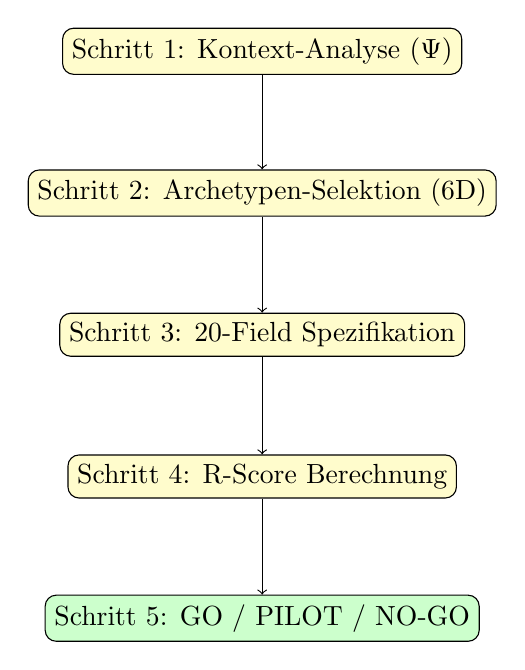
\begin{tikzpicture}[node distance=1.8cm, auto]
\node[draw, rounded corners, fill=yellow!20, minimum width=4cm] (S1) {Schritt 1: Kontext-Analyse ($\Psi$)};
\node[draw, rounded corners, fill=yellow!20, minimum width=4cm, below of=S1] (S2) {Schritt 2: Archetypen-Selektion (6D)};
\node[draw, rounded corners, fill=yellow!20, minimum width=4cm, below of=S2] (S3) {Schritt 3: 20-Field Spezifikation};
\node[draw, rounded corners, fill=yellow!20, minimum width=4cm, below of=S3] (S4) {Schritt 4: R-Score Berechnung};
\node[draw, rounded corners, fill=green!20, minimum width=4cm, below of=S4] (S5) {Schritt 5: GO / PILOT / NO-GO};
\draw[->] (S1) -- (S2);
\draw[->] (S2) -- (S3);
\draw[->] (S3) -- (S4);
\draw[->] (S4) -- (S5);
\end{tikzpicture}
\end{center}

\end{tcolorbox}


\subsection{Schritt 1: Kontext-Analyse}

Bestimme den 8-dimensionalen Kontext-Vektor $\Psi$:

\begin{center}
\begin{tabular}{@{}lll@{}}
\toprule
\textbf{Dimension} & \textbf{Frage} & \textbf{Wert (0--1)} \\
\midrule
$\Psi_E$ & Wie ist die wirtschaftliche Situation? & \\
$\Psi_S$ & Wie stark sind soziale Bindungen? & \\
$\Psi_T$ & Wie viel Zeitdruck besteht? & \\
$\Psi_P$ & Wie ist die physische Umgebung? & \\
$\Psi_I$ & Wie stark sind institutionelle Strukturen? & \\
$\Psi_C$ & Welche kulturellen Faktoren wirken? & \\
$\Psi_D$ & Welche digitale Infrastruktur existiert? & \\
$\Psi_X$ & Welche Umweltfaktoren sind relevant? & \\
\bottomrule
\end{tabular}
\end{center}

\textbf{Zusätzlich charakterisieren:}
\begin{itemize}[nosep]
\item Zielgruppe (Segment aus Appendix PAP1)
\item Aktuelle Journey-Phase (aus Appendix STA)
\item Awareness-Level (aus Appendix AWA)
\end{itemize}


\subsection{Schritt 2: Archetypen-Selektion}

Wähle einen 6D-Vektor basierend auf der Kontext-Analyse:

\begin{equation}
\vec{a} = (\text{Type}, \text{Scope}, \text{Level}, \text{FEPSDE}, \text{Phase}, \text{Awareness})
\end{equation}

\textbf{Prüfe Feasibility:}
\begin{enumerate}[nosep]
\item $C_{\text{affinity}}$: Ist $\alpha_{t,\varphi} \geq 0.4$?
\item $C_{\text{logical}}$: Gibt es logische Widersprüche?
\item $C_{\text{scale}}$: Ist $|s_{\text{rank}} - l_{\text{rank}}| \leq 2$?
\item $\gamma(\Psi)$-Filter: Ist $\gamma(\Psi \rightarrow d) \geq 0.3$?
\end{enumerate}

\textbf{Weise Epistemic Status zu:}
\begin{itemize}[nosep]
\item EMP-Archetype $\rightarrow$ Evidenz für diese Kombination existiert
\item THR-Archetype $\rightarrow$ Theoretisch plausibel, nicht getestet
\item EXP-Archetype $\rightarrow$ Novel, experimentell
\end{itemize}


\subsection{Schritt 3: 20-Field Spezifikation}

Wähle Application Depth (Light/Hybrid/Profound) und fülle die entsprechenden Felder aus.

\textbf{Minimum (Light Mode):}
\begin{itemize}[nosep]
\item F1: Titel
\item F2: Typ
\item F3: Kontext-Level
\item F4: Target Structure
\item F5: FEPSDE Dimension
\item F6: Journey Phase
\end{itemize}


\subsection{Schritt 4: R-Score Berechnung}

Der R-Score (Relevanz-Score) quantifiziert die erwartete Effektivität:

\begin{equation}
R(\vec{a}, \mathcal{K}) = \sum_{i=1}^{n} \alpha_i \cdot \text{Fit}_i(\vec{a}, \mathcal{K})
\label{eq:17-rscore}
\end{equation}

wobei:
\begin{itemize}[nosep]
\item $\alpha_i$ = Gewicht für Fit-Komponente $i$ (aus Appendix CAL1 kalibriert)
\item $\text{Fit}_i$ = Passung zwischen Archetyp und Kontext auf Dimension $i$
\item $\mathcal{K}$ = Kontext-Spezifikation
\end{itemize}

\textbf{Typische Fit-Komponenten:}
\begin{enumerate}[nosep]
\item Phase-Type Affinity
\item Awareness-Match
\item Dimension-Fit
\item Scale-Consistency
\item Resource-Match
\item $\Psi$-Alignment
\end{enumerate}


\subsection{Schritt 5: GO / PILOT / NO-GO Entscheidung}

\begin{tcolorbox}[colback=green!5!white, colframe=green!75!black,
    title=\textbf{Entscheidungsregeln}]

\begin{center}
\renewcommand{\arraystretch}{1.5}
\begin{tabular}{@{}lcll@{}}
\toprule
\textbf{R-Score} & \textbf{Archetype Status} & \textbf{Entscheidung} & \textbf{Aktion} \\
\midrule
$R > 0.7$ & EMP & \cellcolor{green!30}\textbf{GO} & Direkt implementieren \\
$R > 0.7$ & THR/EXP & \cellcolor{yellow!30}\textbf{PILOT} & Mit Messung starten \\
$0.4 < R \leq 0.7$ & Alle & \cellcolor{yellow!30}\textbf{PILOT} & Kleiner Test \\
$R \leq 0.4$ & Alle & \cellcolor{red!30}\textbf{NO-GO} & Nicht implementieren \\
\bottomrule
\end{tabular}
\end{center}

\textbf{Begründung:}
\begin{itemize}[nosep]
\item GO: Hohe Passung + empirische Evidenz → geringes Risiko
\item PILOT: Unsicherheit → vor Scale testen
\item NO-GO: Zu geringe erwartete Wirkung
\end{itemize}

\end{tcolorbox}


%%%%%%%%%%%%%%%%%%%%%%%%%%%%%%%%%%%%%%%%%%%%%%%%%%%%%%%%%%%%%%%%%%%%%%%%%%%%%%%
%%%%%%%%%%%%%%%%%%%%%%%%%%%%%%%%%%%%%%%%%%%%%%%%%%%%%%%%%%%%%%%%%%%%%%%%%%%%%%%
%%  TEIL VI: WORKED EXAMPLES
%%%%%%%%%%%%%%%%%%%%%%%%%%%%%%%%%%%%%%%%%%%%%%%%%%%%%%%%%%%%%%%%%%%%%%%%%%%%%%%
%%%%%%%%%%%%%%%%%%%%%%%%%%%%%%%%%%%%%%%%%%%%%%%%%%%%%%%%%%%%%%%%%%%%%%%%%%%%%%%

\section{Worked Examples}
\label{sec:17-examples}

\subsection{Beispiel 1: Altersvorsorge Auto-Enrollment}
\label{sec:17-example-pension}

\textbf{Kontext:} Eine Pensionskasse will die Teilnahme an der Altersvorsorge unter 25-35-Jährigen erhöhen. Aktuelle freiwillige Teilnahme: 45\%.

\subsubsection{Schritt 1: Kontext-Analyse}

\begin{center}
\begin{tabular}{@{}ll@{}}
\toprule
\textbf{Aspekt} & \textbf{Wert} \\
\midrule
$\Psi_I$ (Institutionell) & 0.8 (hohes Vertrauen in Arbeitgeber) \\
Segment & ``Passive Sparer'' (akzeptieren Defaults) \\
Phase & Trigger (wissen um Wichtigkeit, handeln nicht) \\
Awareness & Medium (A $\approx$ 0.5) \\
\bottomrule
\end{tabular}
\end{center}

\subsubsection{Schritt 2: Archetypen-Selektion}

\begin{equation}
\vec{a} = (\text{Kontextuell}, \text{Tactical}, \text{Individual}, \text{Financial}, \text{Trigger}, \text{Medium})
\end{equation}

\textbf{Feasibility:}
\begin{itemize}[nosep]
\item $\alpha_{\text{Kontextuell, Trigger}} = 0.8$ ✓
\item Keine logischen Widersprüche ✓
\item $|3 - 1| = 2 \leq 2$ ✓
\item $\gamma(\Psi_I = 0.8 \rightarrow F) = 0.6 \geq 0.3$ ✓
\end{itemize}

\textbf{Epistemic Status:} EMP-Archetype (Madrian \& Shea 2001, Chetty et al. 2014)

\subsubsection{Schritt 3: 20-Field Spezifikation (Light Mode)}

\begin{center}
\begin{tabular}{@{}ll@{}}
\toprule
\textbf{Field} & \textbf{Wert} \\
\midrule
F1: Titel & Auto-Enrollment Retirement Default \\
F2: Typ & Kontextuell (Type 3) \\
F3: Kontext & Organizational \\
F4: Target & IND (Future Self) \\
F5: FEPSDE & Financial \\
F6: Phase & Trigger → Action \\
\bottomrule
\end{tabular}
\end{center}

\subsubsection{Schritt 4: R-Score}

\begin{align}
R &= 0.2 \times 0.8 + 0.2 \times 0.7 + 0.2 \times 1.0 + 0.2 \times 1.0 + 0.1 \times 0.9 + 0.1 \times 0.8 \\
&= 0.16 + 0.14 + 0.20 + 0.20 + 0.09 + 0.08 = \mathbf{0.87}
\end{align}

\subsubsection{Schritt 5: Entscheidung}

$R = 0.87 > 0.7$ und EMP-Archetype → \textbf{GO}

\textbf{Erwartetes Ergebnis:} Teilnahme steigt von 45\% auf $\approx$86\% (basierend auf Literatur).


\subsection{Beispiel 2: Energiesparen Portfolio}
\label{sec:17-example-energy}

\textbf{Kontext:} Eine Gemeinde will den Energieverbrauch der Haushalte um 15\% in 3 Jahren senken.

\textbf{Lösung:} Nicht eine Intervention, sondern ein \textbf{kohärentes Portfolio}:

\begin{table}[htbp]
\centering
\small
\begin{tabular}{@{}llllcc@{}}
\toprule
\textbf{Intervention} & \textbf{Typ} & \textbf{Phase} & \textbf{Path Function} & \textbf{$\gamma$} & \textbf{R-Score} \\
\midrule
Soziale Norm Mailings & Sozial & Awareness & Door-opener & --- & 0.72 \\
Smart-Meter Feedback & Feedback & Action & Amplifier & 0.5 & 0.81 \\
Commitment Cards & Bindung & Maintenance & Stabilizer & 0.4 & 0.68 \\
\bottomrule
\end{tabular}
\end{table}

\textbf{Portfolio-Effekt:}
\begin{equation}
E_{\text{Portfolio}} = E_1 + E_2 + E_3 + \gamma_{12}\sqrt{E_1 E_2} + \gamma_{23}\sqrt{E_2 E_3}
\end{equation}

Erwartete Reduktion: 12--15\% (statt 5--8\% mit Einzelintervention).


\subsection{Beispiel 3: Gescheiterte Intervention (Lernbeispiel)}
\label{sec:17-example-failure}

\textbf{Kontext:} Ein Unternehmen will freiwilliges Engagement erhöhen durch Kombination von sozialer Norm (``70\% deiner Kollegen engagieren sich'') und finanziellem Bonus (50 CHF pro Engagement-Tag).

\textbf{Problem:} Die Intervention hat $\gamma_{\text{Sozial, Finanziell}} < 0$ (Crowding-out).

\textbf{Ergebnis:} Engagement sinkt bei intrinsisch motivierten Mitarbeitern. Der finanzielle Bonus signalisiert, dass Engagement eine Transaktion ist, keine moralische Handlung.

\textbf{Lektion:}
\begin{itemize}[nosep]
\item Immer $\gamma$-Matrix prüfen vor Portfolio-Design
\item Incentives nicht mit normativen Interventionen kombinieren bei $\gamma < 0$
\item F10 (Complementarity) im Schema nutzen
\end{itemize}


\subsection{Beispiel 4: Mental Identity Budgeting --- Type Transformation T7$\rightarrow$T5}
\label{sec:17-example-mental-budgets}

\textbf{Kontext:} Ein Unternehmen will Mitarbeiterbindung erhöhen. Problem: Überstunden verfallen nach 6 Monaten---wahrgenommen als Verlust.

\textbf{Innovative Lösung: Type Transformation}

Statt die Überstunden als reinen finanziellen Wert (T7) zu behandeln, werden sie in \textbf{Identity Budgets} (T5) transformiert:

\begin{table}[htbp]
\centering
\caption{Mental Identity Budgets: T7$\rightarrow$T5 Transformation}
\label{tab:17-mental-budgets}
\renewcommand{\arraystretch}{1.3}
\small
\begin{tabular}{@{}llll@{}}
\toprule
\textbf{Budget} & \textbf{Identitäts-Dimension} & \textbf{Ziel-Segment} & \textbf{$\sigma$} \\
\midrule
Community & ``Contributor / Giver'' & social\_oriented & 1.6 \\
Care & ``Caregiver / Protector'' & loss\_averse & 1.4 \\
Sabbatical & ``Self-Investor'' & autonomy\_seeking & 1.5 \\
Learning & ``Expert / Learner'' & sophisticates & 1.3 \\
\bottomrule
\end{tabular}
\end{table}

\textbf{Mechanismus:}
\begin{equation}
\text{Überstunden (T7: } u_F\text{)} \xrightarrow{\text{Reframing}} \text{Identity Budgets (T5: } W_{\text{base}}\text{)}
\end{equation}

\textbf{Warum funktioniert das?}
\begin{enumerate}[nosep]
\item \textbf{Crowding-Out vermieden:} T5 hat keine negativen $\gamma$ mit anderen Typen
\item \textbf{Alle Segmente aktiviert:} Jedes Segment findet ``sein'' Budget ($\sigma > 1.0$ für alle)
\item \textbf{Autonomie erhöht:} Mitarbeiter wählen selbst $\rightarrow$ geringe Reaktanz
\item \textbf{Identity Lock-In:} Bei Austritt ``verliert'' man aufgebaute Identität
\end{enumerate}

\textbf{20-Field Spezifikation (Auszug):}
\begin{center}
\begin{tabular}{@{}ll@{}}
\toprule
\textbf{Field} & \textbf{Wert} \\
\midrule
F1: Titel & Overtime Mental Budgets System \\
F2: Typ & T5 (Identity), \textit{secondary:} T7 (transformed) \\
F5: FEPSDE & Social (0.5), Development (0.2), Financial (0.1) \\
F6: Phase & Maintenance $\rightarrow$ Stable ($\alpha = 0.8, 0.9$) \\
F8: Autonomie & Voluntary, Reactance Risk = very\_low \\
F9: Segment & All segments (via segment\_budget\_affinity) \\
F10: $\gamma$ & $+0.3$ mit T1, $+0.2$ mit T2, keine Konflikte \\
\bottomrule
\end{tabular}
\end{center}

\textbf{Exit-Regel (Identity Lock-In):}

Bei Kündigung greift ein \textbf{Identity Discount} (z.B.\ 50\%):
\begin{equation}
\text{Auszahlung} = \text{Stunden} \times \text{Stundensatz} \times (1 - \delta_{\text{identity}})
\end{equation}

\textit{Rationale:} ``Die Stunden hatten einen Identitätswert \textit{hier}---dieser Wert ist an diese Gemeinschaft gebunden.''

\textbf{Lektion:}
\begin{itemize}[nosep]
\item Type Transformation (T7$\rightarrow$T5) kann Crowding-Out vermeiden
\item Multiple Budget-Optionen erhöhen Autonomie und reduzieren Reaktanz
\item Identity Lock-In schafft Switching Costs ohne klassische ``Golden Handcuffs''
\item Segment-Budget-Affinity ermöglicht One-System-fits-All Design
\end{itemize}

\begin{tcolorbox}[colback=blue!5!white, colframe=blue!75!black]
\textbf{Advanced Pattern:} Mental Identity Budgeting zeigt, dass die 8 Interventionstypen nicht statisch sind---durch geschicktes Reframing kann monetärer Wert in Identitätswert transformiert werden, was neue Portfolio-Möglichkeiten eröffnet.
\end{tcolorbox}


%%%%%%%%%%%%%%%%%%%%%%%%%%%%%%%%%%%%%%%%%%%%%%%%%%%%%%%%%%%%%%%%%%%%%%%%%%%%%%%
%%%%%%%%%%%%%%%%%%%%%%%%%%%%%%%%%%%%%%%%%%%%%%%%%%%%%%%%%%%%%%%%%%%%%%%%%%%%%%%
%%  TEIL VII: ZUSAMMENFASSUNG UND READING PATH
%%%%%%%%%%%%%%%%%%%%%%%%%%%%%%%%%%%%%%%%%%%%%%%%%%%%%%%%%%%%%%%%%%%%%%%%%%%%%%%
%%%%%%%%%%%%%%%%%%%%%%%%%%%%%%%%%%%%%%%%%%%%%%%%%%%%%%%%%%%%%%%%%%%%%%%%%%%%%%%

\section{Summary}
\label{sec:17-summary}

\begin{tcolorbox}[colback=green!5!white, colframe=green!75!black,
    title=Key Points]

\begin{enumerate}
\item \textbf{Emergenz:} Die Interventionslogik emergiert systematisch aus dem 10C Framework:
\begin{equation}
\text{10C} \rightarrow \text{6D} \rightarrow 14{,}400 \rightarrow \gamma(\Psi)\text{-Filter} \rightarrow \approx 2{,}000
\end{equation}

\item \textbf{8 Typen:} Alle Interventionen lassen sich auf 8 primitive Typen zurückführen, die aus der $W_{\text{eff}}$-Zerlegung emergieren.

\item \textbf{20-Field Schema:} Standardisierte Spezifikation mit drei Tiers (Emergent, Operational, Interface) und drei Depths (Light, Hybrid, Profound).

\item \textbf{5 Dimensionen:} TYPE, PHASE, SEGMENT, PORTFOLIO, CONTEXT---jede erfordert spezifische Entscheidungen.

\item \textbf{5-Schritt Prozess:} Kontext → Archetyp → Spezifikation → R-Score → GO/PILOT/NO-GO

\item \textbf{Epistemische Ehrlichkeit:} Unterscheide EMP/THR/EXP-Archetypen und dokumentiere Annahmen (A1--A7).
\end{enumerate}

\end{tcolorbox}

\begin{tcolorbox}[colback=blue!5!white, colframe=blue!75!black,
    title=Der Interventions-Workflow auf einen Blick]

\begin{center}
\texttt{Kontext ($\Psi$) → 6D-Archetyp → Feasibility → 20-Field → R-Score → Entscheidung}
\end{center}

\end{tcolorbox}

%------------------------------------------------------------------------------
\paragraph{Formal Details.}
Die vollständige formale Behandlung findet sich in Appendix~HHH (METHOD-TOOLKIT), welcher enthält:
\begin{itemize}[nosep]
\item 8 Theoreme (HHH-T1 bis T8) für die 10C $\rightarrow$ HHH Emergence
\item 5 Definitionen (HHH-D1 bis D5) für Archetyp-Klassifikation
\item 3 Axiome (HHH-A1 bis A3) für epistemische Ehrlichkeit
\item 4 Forschungsfragen (RQ-1 bis RQ-4) für Tier-2 Emergence
\end{itemize}
Zusätzlich: Appendix~III (METHOD-LLMMC-CAL) für R-Score Kalibrierung und GO/PILOT/NO-GO Schwellenwerte.

%------------------------------------------------------------------------------
\paragraph{What Comes Next.}
Die folgenden Kapitel vertiefen spezifische Dimensionen der Interventionslogik:
\begin{itemize}[nosep]
\item \textbf{Kapitel 18} führt die \textbf{Journey-Integration} ein---wie Interventionen über Zeit sequenziert werden.
\item \textbf{Kapitel 19} behandelt \textbf{Segment-Spezifität}---wie Interventionen an Zielgruppen angepasst werden.
\item \textbf{Kapitel 20} entwickelt das \textbf{Portfolio-Design}---wie Interventionen optimal kombiniert werden.
\end{itemize}

%------------------------------------------------------------------------------

\subsection{Was dieses Kapitel NICHT abdeckt}

Dieses Kapitel ist das \textbf{Master-Kapitel}. Die folgenden Kapitel vertiefen spezifische Aspekte:

\begin{itemize}
\item \textbf{Kapitel 18: Journey-Integration} --- Wie wähle ich die richtige Phase? Wie sequenziere ich über Zeit?
\item \textbf{Kapitel 19: Segment-Spezifität} --- Wie passe ich an verschiedene Zielgruppen an? Wie manage ich Reaktanz?
\item \textbf{Kapitel 20: Portfolio-Design} --- Wie kombiniere ich Interventionen optimal? Wie vermeide ich Crowding-out?
\end{itemize}


\subsection{Reading Path}
\label{sec:17-reading-path}

\begin{tcolorbox}[colback=gray!5!white, colframe=gray!75!black,
    title=Empfohlene Lesepfade]

\textbf{Für Praktiker:}
\begin{enumerate}[nosep]
\item Dieses Kapitel (Gesamtlogik)
\item Kapitel 18 (wenn Journey-Fokus)
\item Kapitel 19 (wenn Segment-Fokus)
\item Kapitel 20 (wenn Portfolio-Fokus)
\end{enumerate}

\textbf{Für Forscher:}
\begin{enumerate}[nosep]
\item Appendix HHH (vollständige Theoreme)
\item Appendix CAL1 (R-Score Kalibrierung)
\item Dann Kapitel 17--20
\end{enumerate}

\textbf{Für Einsteiger:}
\begin{enumerate}[nosep]
\item Section~\ref{sec:17-types} (8 Typen verstehen)
\item Section~\ref{sec:17-examples} (Beispiele durcharbeiten)
\item Dann Rest des Kapitels
\end{enumerate}

\end{tcolorbox}


% =============================================================================
% POLICY IMPLICATIONS (Required for Type C chapters)
% =============================================================================

\section*{Policy Implications}

\begin{enumerate}
\item \textbf{Für Regierungen:} Nutze das 20-Field Schema für alle Behavioral Policy Interventionen. Dokumentiere systematisch für organisationales Lernen.

\item \textbf{Für Unternehmen:} Implementiere den 5-Schritt Prozess für HR-, Marketing- und Change-Interventionen. Prüfe immer die $\gamma$-Matrix vor Portfolio-Design.

\item \textbf{Für NGOs:} Beginne mit Light Mode für rapid prototyping, iteriere zu Profound Mode für Scale-up.

\item \textbf{Für Forscher:} Die offenen Forschungsfragen RQ-1 bis RQ-4 (Appendix HHH) bieten Ansatzpunkte für Tier-2 Emergence-Formalisierung.
\end{enumerate}


% =============================================================================
% END OF CHAPTER
% =============================================================================
